\documentclass[12pt]{extarticle}
\usepackage[utf8]{inputenc}
\usepackage{cite}
\usepackage{url}
\usepackage{graphicx}
\usepackage{float}
\graphicspath{ {./figs/} }

\title{Quantification of Uncertainty in Medical Image Segmentation}
\author{Hao Wang, Yunhao Luo}
\date{October 2020}

\begin{document}

\maketitle
\section*{Abstract}
\textbf{TODO}
\section{Introduction}
\paragraph{}
Recent development of deep learning algorithms has greatly contributed to
the performance gain on natural image analysis, of which lots
of algorithms has been proposed to address image classification and semantic
segmentation problems and large-scale datasets with abundant annotations have been
carried out\cite{nair_precup_arnold_arbel_2020}.
However, due to
% inter-reader variations need more details and background
both lack of annotations and high inter-reader variations\cite{zhang2020disentangling}
in medical domain, the application of deep models on clinical diagnosis,
which is known to be sensitive to false-positive and true-negative cases that may leads
to severe consequences, is still a challenging problem.
For instance, the inter-annotator difference of glioblastoma segmentation
is pointed out to be in the range of 74-84\% \cite{6975210}.
Researches on inter-observer variance also found out
the large and wide-existing inconsistency among annotations of biomedical structures
\cite{Variability2019}\cite{interobserver2018}. Such high-variance dataset 
could result in poor performance of supervised machine learning algorithms,
which are known to be highly dependent on the quality of data as well as their annotations.
To overcome it, the most straight-forward and widely-adopted method 
is to take the majority vote of experts' annotations, treating every 
experts' opinions equally significant\cite{6975210}, while STAPLE proposed by \cite{STAPLE} 
evaluates reliability of annotators and assigns weights to each of them when 
fusing annotations accordingly. Both of the approaches focus on per image annotation fusion
while ignoring information across the whole dataset\cite{zhang2020disentangling}.
Lately, a challenge about quantification of uncertainty 
in biomedical image segmentation has been carried
out on the purpose of seeking measures to quantify the uncertainty of 
medical image annotation. A discrete approximation of the uncertainty is also
proposed for the assessment of participants' results, which
takes in the averaged ground truth and the provided predicted probability map of a task
and computes and averages the dice score of the threshold of them with
discrete threshold values\cite{qubiq} that could be considered as 
measuring the quality of the predicted cumulative probability map in a discrete manner. 
A high averaged dice score is then considered to be an indication of 
good quantification of the inter-observer uncertainty.
Therefore, our goal is to firstly follow the QUBIQ challenge and quantify the level of 
uncertainties in biomedical image segmentation. 
Then, since taking threshold averaged dice score treats certain and uncertain pixels equally 
and ignores the fact that most uncertain pixels lies around 
the contour of the lesion area, we are expecting to have a
better evaluation method for inter-reader variations as well as objective function for 
optimization. Finally, based on the metrics we derive, a further
optimized method could be explored and proposed.
\section{Related Works}
\paragraph{}
Uncertainty in deep learning can be inclusively divided into \textit{Aleatoric}
uncertainty and \textit{Epistemic} uncertainty \cite{kendall2017uncertainties}.
\textit{Aleatoric} uncertainty or data uncertainty typically occurs during data sampling and
observation error of observer and is irreducible even feeded with more data, which shares a
close connection with inter-observer variations. As for \textit{epistemic}
uncertainty, it refers to ambiguity of model prediction that can be reduced by feeding abundant data.
An example of it is that a model trained on only part of a dataset may over-confidently
predict unseen data into wrong classes. Recent development on 
bayesian neural network has made it possible to quantify the 
uncertainty of model prediction by replacing scalar parameters with distributions such 
that outputs' variance reflects the predictive uncertainty of the model since parameters are now sampled 
from a `pre-defined" prior distribution, which could be considered a 
combination of \textit{aleatoric} uncertainty and \textit{epistemic} uncertainty 
and can be divided into two parts by the law of total variance with each part corresponding to 
one of the uncertainties. It could also be exploited to estimate \textit{aleatoric} uncertainty by 
minimizing the \textit{epistemic} uncertainty. \cite{kohl2019probabilistic} 
proposed a method that involves uncertainties by deploying variational 
auto-encoder(VAE) into U-Net, the widely used model in medical image segmentation\cite{ronneberger2015unet}. 
The VAE here accounts for variations of annotations and represents an 
estimation of joint distribution that includes every pixels of the segmentation map. 
The framework is capable of providing multiple segmentation 
hypothesis with each of them estimating the knowledge of one expert.
However, the drawbacks of the bayesian approach are of the extra computation
,excessive training time and implementation difficulty. 
Some recent studies proposed to use a dropout network, during the testing stage of which, 
the dropout is kept, predictions are sampled using Monte Carlo methods 
and various uncertainties are computed based on the sampled results.
It is also reported that Effective performance can be achieved 
without any additional parameters even compared with non-bayesian methods. 
However, for such methods, the ambiguity obtained is
% Aleatoric & Epistemic uncertainty needs more explanation
not a direct representation of the \textit{Aleatoric} uncertainty(the noise of data)
, but \textit{epistemic} uncertainty in model
\cite{kendall2017uncertainties}. Therefore, the resulted uncertainty could not
be treated as the inter-reader variability but the reliability of 
the model itself when only insufficient data is provided. 
\cite{nair_precup_arnold_arbel_2020}. 
\paragraph{}
Another study by \cite{zhang2020disentangling} used confusion matrices to
model each annotator. They hold the assumption that there is one and
only one ground truth annotation for an input of certain task settings and
that annotations are noised approximation of the ground truth
, which can be obtained by matrix multiplication of annotators' 
confusion matrices with ground truth. Then, with two convolution neural network backbone
where one outputs the estimated ground truth and the other accounts for the confusion matrices
of each annotator, and by forcing the matrix multiplication of them to be similar to the
real annotation, a unique ground truth could be learned by optimizing the cross entropy term
and another regularization term that minimizes the trace of the confusion matrices.
Though the inter-observer variance is not directly measured, the well-modeled annotators'
confusion matrices could be utilized to produce further results
as well as measurements of uncertainties.
Nevertheless, the correctness of the assumption of this approach
still remains to be verified and evaluated since there's no dataset available 
that fulfils their requirement by the publish time of their work.
\paragraph{}
To accurately model the multiple annotator variability, Shi Hu et al.\cite{hu2019supervised} utilized the multiple annotator dataset
to form a `ground truth" for aleatoric uncertainty. Then a supervised framework for estimating
as well as qualifying \textit{aleatoric} uncertain is proposed and combined with probabilistic U-Net
to produce fine-grained uncertainty approximations. 

\section{Planned Method}
\begin{figure}[ht!]
\centering
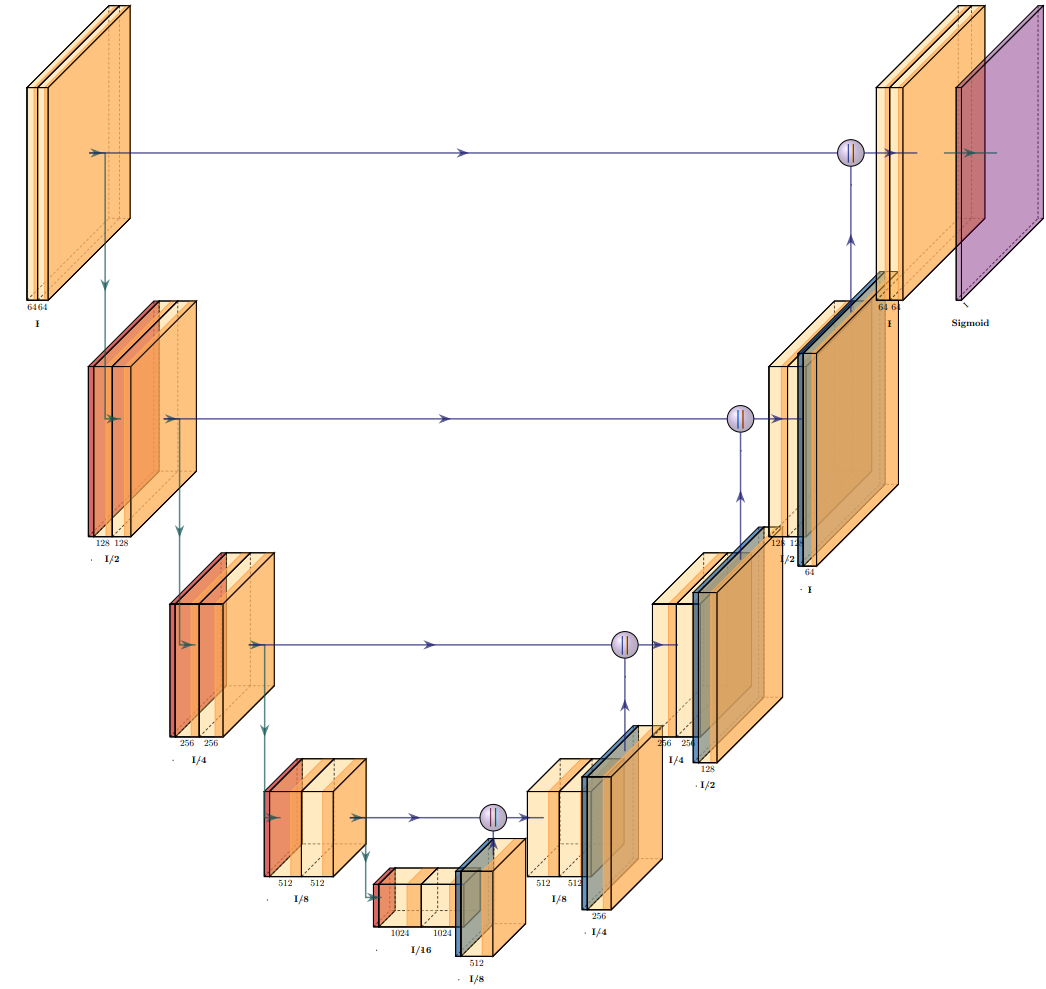
\includegraphics[scale=0.28]{fig2.png}
\caption{U-Net architecture\cite{iqbal_2018}}
\label{pre_results}
\end{figure}
\begin{figure}[ht!]
\centering
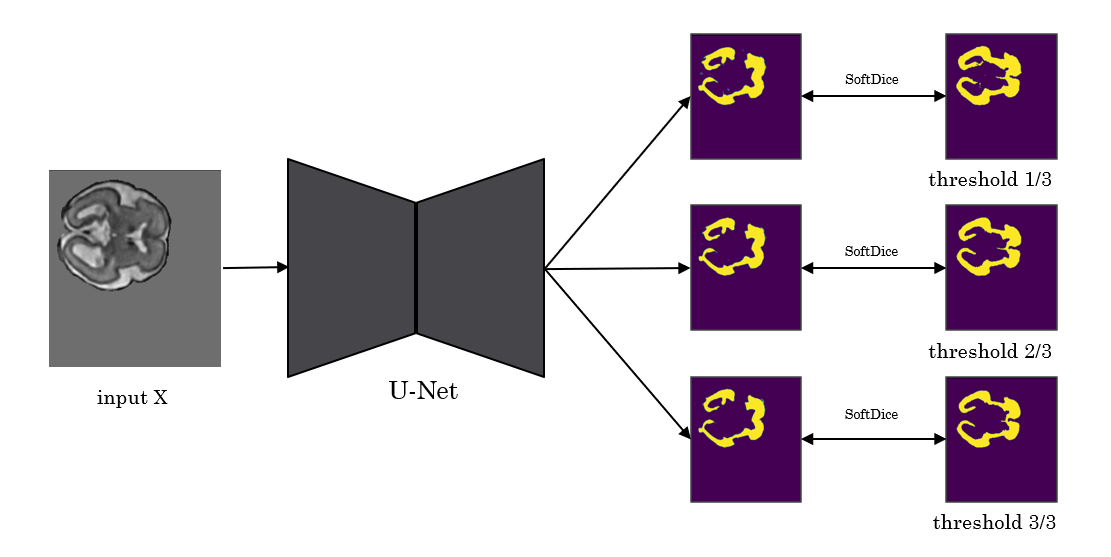
\includegraphics[scale=0.25]{fig3.png}
\caption{Our baseline method}
\label{proposed_mothod}
\end{figure}
\paragraph{}
To model the inter-observer variability in the segmentation task, 
the most straight-forward way is to directly estimate the annotations
 by each experts separately, with each channels of the probability 
 map output of the deep model representing them, respectively. 
 However, since dice coefficient loss and cross entropy 
assign equal weights to every target area, the area around the contour, 
which has the most disagreement among experts, won't be handled carefully\cite{Kervadec_2021}.
The second thought is to follow the metric given by \cite{qubiq} and directly 
optimize on it by estimating threshold result of the averaged segmentation map 
at threshold value of $\frac{1}{M}, \frac{2}{M}, ..., \frac{M}{M}$, 
where $M$ is the number of annotators. A preliminary result is obtained and 
shown in section 4 using this method and U-Net as backbone model.
\begin{equation}
    y_{p} = \{y_{p\frac{1}{M}}, y_{p\frac{2}{M}}, ... y_{p\frac{M-1}{M}},y_{p\frac{M}{M}}\}
\end{equation}
\begin{equation}
    y_{g} = \{y_{g\frac{1}{M}}, y_{g\frac{2}{M}}, ... y_{g\frac{M-1}{M}},y_{g\frac{M}{M}}\}
\end{equation}
\begin{equation}
    L = 1 - \frac{1}{NM}\sum_{n=1}^{N}\sum_{m=1}^{M}SoftDice(y_{p\frac{m}{M}}^{(n)}, y_{g\frac{m}{M}}^{(n)})
\end{equation}
\begin{equation}
    SoftDice(y_p, y_g) = \frac{2\sum y_p y_g}{\sum y_p +  \sum y_g + \epsilon}
\end{equation}
where $y_p$ is the prediction with each
channel representing an estimation of binary segmentation map at multiple threshold values, 
$y_g$ the ground truth binary segmentation map with corresponding threshold 
values as $y_p$ and $\epsilon$ is the smooth factor that smooths 
the training process by avoiding fluctuation caused by division of small value.
$L$ is the loss function that maximizes the similarity 
between $y_p$ and $y_g$ using soft dice coefficient 
to be optimized with stochastic gradient descend. 
\paragraph{}
Another direction would be to follow the idea of 
\cite{zhang2020disentangling} and \cite{kohl2019probabilistic}, 
dividing the architecture into two components. 
While one accounts for generating estimated `ground truth" segmentation map,
the other models annotators in a unified or separated manner. By combining 
the two components, a consistent segmentation result based on each annotator 
could be obtained and various uncertainty metrics could be adopted for
the evaluation of the correctness of the uncertainty. For example,
since the desired \textit{aleatoric} uncertainty can be 
estimated given the annotations of an image annotated by multiple experts\cite{qubiq}, 
by quantifying the difference between the ground truth uncertainty and 
the uncertainty computed out of the prediction, we can measure the goodness and the correctness of
results. On top of that, an objective function targeted at 
minimizing the difference could be adopted. The only problem would be the 
extremely small amount of data, which may lead to high \textit{epistemic} uncertainty and 
poor estimates of \textit{aleatoric}(the desired uncertainty). Therefore, the key of this approach 
is to properly handle the difficulties caused by insufficient data.

\section{Preliminary Results and Analysis}
\begin{figure}[ht!]
\centering
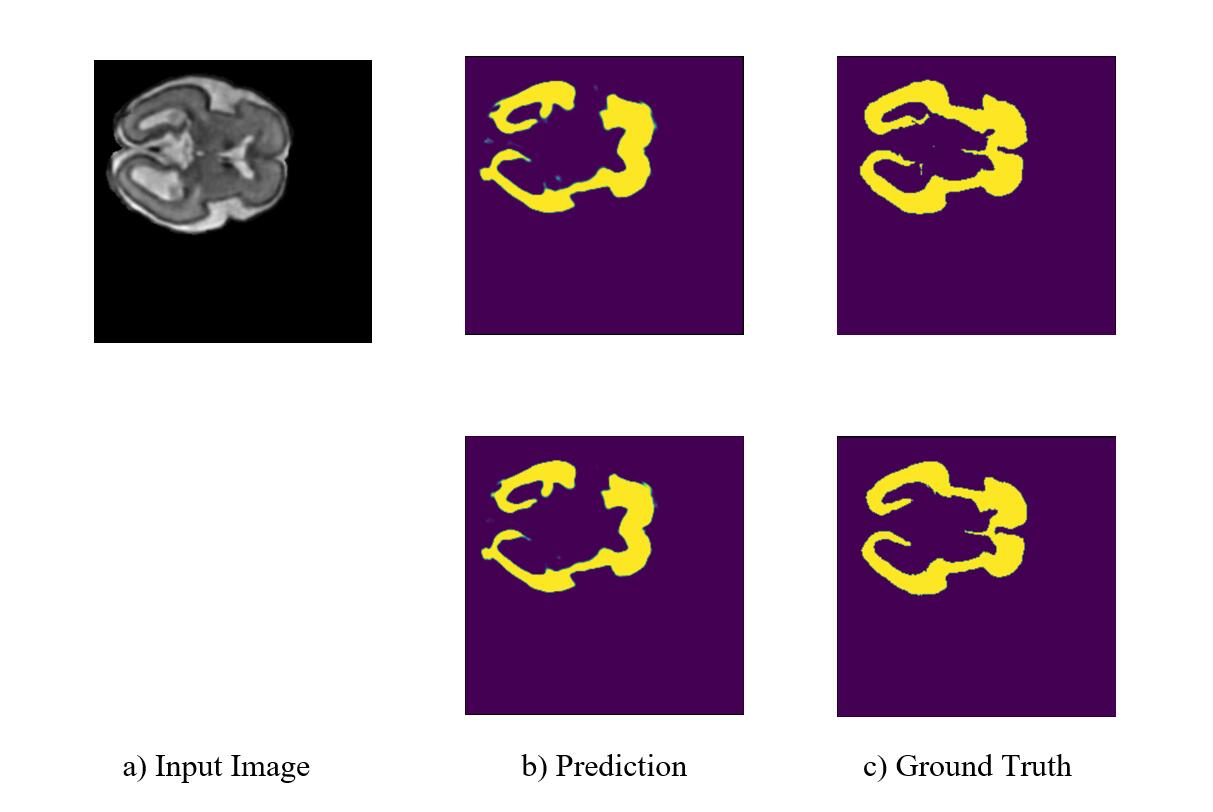
\includegraphics[scale=0.28]{fig1.jpg}
\caption{The results of \textit{Brain Growth} task on the validation set of 
QUBIQ dataset with 7 annotators. a) is the brain 
MRI scan of a participant. b) is the predicted sigmoid output. The top row represents output at threshold  
value of $\frac{1}{7}$ and the bottom one represents output at threshold value of $\frac{2}{7}$. c) is the 
ground truth segmentation map at same threshold values with b).}
\label{U-Net}
\end{figure}
\paragraph{}
This part we demonstrate some of the preliminary results obtained on the QUBIQ uncertainty dataset.
The result shown in Figure \ref{pre_results} is obtained using the method mentioned in the previous 
section without pre-training nor data augmentation, which has 
a averaged dice score of 0.7702 under the evaluation metric of the challenge. 
Though it could be considered a medium-level result for a segmentation task, especially for such
a small amount of data samples, as for uncertainty, most of the uncertain pixels around the contour area are not 
correctly approximated, which reflects the weakness of the objective of 
being not focused enough on uncertain data point or could be considered a high \textit{epistemic} uncertainty. 
Larger weights should be assigned to those pixels with high inter-reader variability. Pretraining on 
related single annotator dataset may also help reduce the difference between 
prediction and ground truth discrete \textit{aleatoric} uncertainty.
\section{Evaluation Metrics}
\paragraph{}
Based on the metric provided by \cite{qubiq}, a naive evaluation of our result could be given by:
\begin{equation}
    S = \frac{1}{TNH}\sum_{t=1}^{T}\sum_{n=1}^{N}\sum_{h=1}^{H}DiceCoef(y_{p\frac{h}{H}}^{(t)}, y_{g\frac{h}{H}}^{(t)})
\end{equation}
where T is total number of tasks, N is the size of the validation set and H refers to 
the number of threshold values. It could be considered a discrete estimation of quality of the cumulative probability 
distribution.
\paragraph{}
To further explore the quality \textit{aleatoric} uncertainty as well as the accuracy and sample diversity, we plan to 
adopt the generalized energy distance metric, that has the form:
\begin{equation}
    D^2_{GED} = 2E[d(S, Y)] - E[d[S, S']] - E[d(Y, Y')]
\end{equation}
\begin{equation}
    d(A, B) = 1 - IoU(A, B)
\end{equation}
where S is samples from the bayesian model or Monte Carlo dropout model, Y is the corresponding 
annotations. The first term of GED accounts for the difference between sampled predictions
and annotations. The rest terms quantify the expected difference of the sampled predictions and 
annotations among themselves. 

% TODO
% Problem Formulation
% \begin{enumerate}
%    \item Achieve high performance under QUBIQ evaluation metrics.
%    \item Define a better metric for the assessment of uncertainties in medical image segmentation.
%    \item Derive a method for the measurement of data uncertainties.
%    \item Address uncertainties caused by inter-reader variations.
%\end{enumerate}

\bibliographystyle{plain}
\bibliography{M335}

\end{document}
